\documentclass[../main.tex]{subfiles}

\begin{document}
\section{Proofs}\label{sec:proofs_appendix}
\subsection{Conics in a nutshell}
\begin{proposition}
  The area enclosed in an ellipse of semi-major axis $a$ and semi-minor axis $b$ is $\pi a b$.
\end{proposition}
\begin{proof}
  Consider the ellipse $E$ centered at the origin and oriented as in \cref{fig:circle-ellipse}.
  \begin{figure}[htbp]
    \centering
    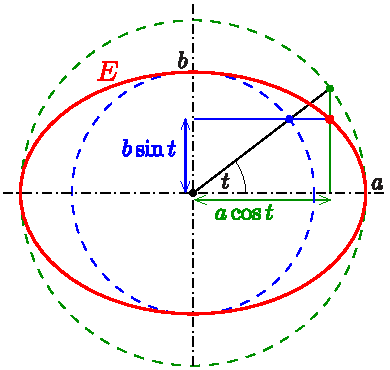
\includegraphics[width=0.5\textwidth]{Images/circles-ellipse.pdf}
    \caption{Reference frame centered at the center of the ellipse. Source: \cite{wiki:conic-ellipse}.}
    \label{fig:circle-ellipse}
  \end{figure}

  From \cref{fig:circle-ellipse} one can check that it can be parametrized by $(x,y)=(a\cos t,b\sin t)$ with $ t\in[0,2\pi)$. This parametrization satisfies:
  \begin{equation}
    \frac{x^2}{a^2}+\frac{y^2}{b^2}=1
  \end{equation}
  Hence, the area enclosed in the ellipse can be parametrized by $(x, y)=(ar\cos t,br\sin t)$, with $r\in[0,1]$ and $t\in[0,2\pi)$. The Jacobian of this transformation is $abr$. Therefore, from the change of variable theorem we have that:
  \begin{equation}
    \mathrm{Area}(E)=\iint_E\dd{x}\dd{y}=\int_{0}^{2\pi}\int_{0}^{1}abr\dd{r}\dd{t}=\pi ab
  \end{equation}
\end{proof}
\subsection{Introduction to astrodynamics and satellite tracking}
\begin{proposition}[Kepler's first law]
  \label{prop:two-body}
  Consider two point-mass bodies. The motion of one body orbiting the other can be described by a conic section. Hence, it can be expressed in the form:
  \begin{equation}
    \label{eq:r_conic}
    r(t)=\frac{p}{1+e\cos (\nu(t))}=\frac{h^2/\mu}{1+(B/\mu)\cos(\nu)}
  \end{equation}
  for some parameters $p=h^2/\mu$, $e=B/\mu$ and $B$.
\end{proposition}
\begin{proof}
  Cross-multiplying \cref{eq:Newton} by $\vf{h}$ we obtain
  \begin{equation}
    \dv{(\dot{\vf{r}}\times\vf{h})}{t}=\ddot{\vf{r}}\times\vf{h}=-\frac{\mu}{r^3}\vf{r}\times\vf{h}=-\frac{\mu}{r^3}\vf{r}\times(\vf{r}\times \dot{\vf{r}})=\frac{\mu}{r^3}[(\vf{r}\cdot{\vf{r}})\dot{\vf{r}}-(\vf{r}\cdot\dot{\vf{r}})\vf{r}]
  \end{equation}
  where in the last equality we have used the vector equality $\vf{u}\times(\vf{v}\times\vf{w})=(\vf{u}\cdot\vf{w})\vf{v}-(\vf{u}\cdot\vf{v})\vf{w}$ for $\vf{u}, \vf{v}, \vf{w}\in\RR^3$. Now note that:
  \begin{equation}
    \dv{}{t}\left(\frac{\vf{r}}{r}\right)=\frac{\dot{\vf{r}}}{r}-\frac{\dot{r}}{r^2}\vf{r}= \frac{1}{r^3}[(\vf{r}\cdot{\vf{r}})\dot{\vf{r}}-(\vf{r}\cdot\dot{\vf{r}})\vf{r}]
  \end{equation}
  because\footnote{Bear in mind that in general $\dot{r}\ne\norm{\dot{\vf{r}}}$. Indeed, if $\beta$ denotes the angle between $\vf{r}$ and $\dot{\vf{r}}$ we have that $\dot{r}=\norm{\dot{\vf{r}}}\cos\beta$. In particular $\dot{r}$ may be negative.} $\displaystyle 2r\dot{r}=\dv{(r^2)}{t}=\dv{(\vf{r}\cdot\vf{r})}{t}=2\vf{r}\cdot\dot{\vf{r}}$. Thus:
  \begin{equation}
    \dv{(\dot{\vf{r}}\times\vf{h})}{t}=\mu \dv{}{t}\left(\frac{\vf{r}}{r}\right)
  \end{equation}
  Integrating with respect to the time yields
  \begin{equation}
    \dot{\vf{r}}\times \vf{h}=\frac{\mu}{r}\vf{r}+\vf{B}
  \end{equation}
  where $\vf{B}\in\RR^3$ is the constant of integration. Observe that since $\dot{\vf{r}}\times\vf{h}$ is perpendicular to $\vf{h}$, $\dot{\vf{r}}\times\vf{h}$ lies on the orbital plane and so does $\vf{r}$. Hence, $\vf{B}$ lies on the orbital plane too. Now, dot-multiplying this last equation by $\vf{r}$ and using that $\vf{u}\cdot(\vf{v}\times\vf{w})=(\vf{u}\times\vf{v})\cdot\vf{w}$ $\forall\vf{u},\vf{v},\vf{w}\in\RR^3$ we obtain
  \begin{equation}
    h^2=\vf{h}\cdot\vf{h}=(\vf{r}\times\dot{\vf{r}})\cdot\vf{h}=\vf{r}\cdot(\dot{\vf{r}}\times\vf{h})=\frac{\mu}{r}\vf{r}\cdot\vf{r}+\vf{r}\cdot\vf{B}=\mu r+rB\cos\nu
  \end{equation}
  where $h:=\norm{\vf{h}}$, $B:=\norm{\vf{B}}$ and $\nu$ denotes the angle between $\vf{r}$ and $\vf{B}$, called \emph{true anomaly}. Rearranging the terms we finally obtain the equation of a conic section
  \begin{equation}
    r=\frac{h^2/\mu}{1+(B/\mu)\cos(\nu)}
  \end{equation}
  with $p:=h^2/\mu$ and $e:=B/\mu$.
\end{proof}
\begin{proposition}[Kepler's second law]
  The areal velocity remains constant. In particular:
  \begin{equation}
    \dv{A(t)}{t}=\frac{h}{2}
  \end{equation}
\end{proposition}
\begin{proof}
  Recall that the area of a parallelogram generated by two vectors $\vf{u},\vf{v}\in\RR^3$ is given by $\norm{\vf{u}\times\vf{v}}$. Thus, approximating the difference $A(t+k)-A(t)$ by half of the area of the parallelogram generated by $\vf{r}(t)$ and ${\vf{r}}(t+k)$ (see \cref{fig:areal_vel}) we obtain:
  \begin{multline}
    \dv{A(t)}{t}=\lim_{k\to 0}\frac{A(t+k)-A(t)}{k}=\lim_{k\to 0}\frac{\norm{\vf{r}(t)\times\vf{r}(t+k)}}{2k}=\lim_{k\to 0}\frac{\norm{\vf{r}(t)\times(\vf{r}(t+k)-\vf{r}(t))}}{2k}=\\
    =\frac{\norm{\vf{r}(t)\times\dot{\vf{r}}(t)}}{2}=\frac{h}{2}
  \end{multline}
  where the penultimate equality is due to the continuity and linearity of the cross product.
  \begin{figure}[htbp]
    \centering
    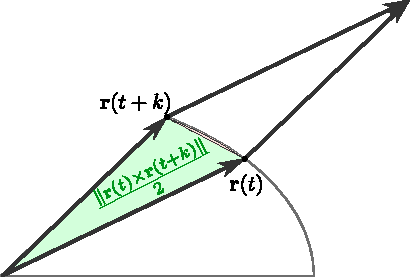
\includegraphics[width=0.5\textwidth]{Images/areal_velocity.pdf}
    \caption{Graphical representation of the error made (red region) when approximating the area swept by the radius vector by half the area of the parallelogram generated by $\vf{r}(t)$ and $\vf{r}(t+k)$ (green region).}
    \label{fig:areal_vel}
  \end{figure}
\end{proof}
\begin{proposition}[Kepler's third law]
  The mean motion is related to the semi-major axis by:
  \begin{equation}
    n=\sqrt{\frac{\mu}{a^3}}
  \end{equation}
\end{proposition}
\begin{proof}
  Integrating \cref{eq:areal_velocity} with respect to time between 0 and $T$ (the period) yields:
  \begin{equation}
    \pi a b=A(T)=\int_0^T A'(t)\dd{t}=\int_0^T \frac{h}{2}\dd{t}=\frac{hT}{2}\implies n=\frac{2\pi}{T}=\frac{h}{a b}=\frac{h}{a^2\sqrt{1-e^2}}=\sqrt{\frac{\mu}{a^3}}
  \end{equation}
  where we have used \cref{eq:semi-major_axis,eq:ellipse_b_a}.
\end{proof}
\begin{lemma}
  Let $e\in[0,1)$, $M\in\RR$ and $\bar{M}=M\mod{2\pi}$ be such that $\bar{M}\in[0,2\pi)$. Then, the function
  \begin{equation}
    f(E) = E-e\sin E - M
  \end{equation}
  has a unique solution in the interval $[M, M+e]$ if $\bar{M}\in[0,\pi)$ and in the interval $[M-e, M]$ if $\bar{M}\in[\pi,2\pi)$.
\end{lemma}
\begin{proof}
  We first prove the uniqueness. Clearly $f\in\mathcal{C}^1(\RR)$ and $f'(E)=1-e\cos E> 0$ for all $E\in[0,2\pi)$ because $e<1$. Thus, $f$ is strictly increasing and so it has at most one zero. Now, if $0\leq \bar{M}< \pi$, then:
  \begin{equation}
    f(M)=-e\sin M\leq 0\qquad\text{ and }\qquad f(M+e)=e(1-\sin (M+e))\geq 0
  \end{equation}
  So by Bolzano's theorem, $f$ has a solution in $[M,M+e]$. If $\pi\leq \bar{M}< 2\pi$, then:
  \begin{equation}
    f(M)=-e\sin M\geq 0\qquad\text{ and }\qquad f(M-e)=-e(1+\sin (M-e))\leq 0
  \end{equation}
  So again by Bolzano's theorem, $f$ has a solution in $[M-e,M]$.
\end{proof}
\subsection{Earth's gravitational field and other perturbations}
\begin{theorem}
  Let $\Omega$ be a compact region in $\RR^3$ with a continuous density of mass $\rho:\Omega\to\RR$. Then, the gravitational acceleration field $\vf{g}$ is conservative. That is, there exists a function $f:\RR^3\rightarrow\RR$ such that $\vf{g}=\grad f$.
\end{theorem}
\begin{proof}
  An easy computation shows that fixed $\vf{s}\in\RR^3$ we have:
  \begin{equation}
    \grad\left(\frac{1}{\norm{\vf{r}-\vf{s}}}\right)=-\frac{1}{\norm{\vf{r}-\vf{s}}^3}(\vf{r}-\vf{s})
  \end{equation}
  So we need to justify whether the following exchange between the gradient and the integral is correct:
  \begin{equation}
    \vf{g}=-\int_{\Omega}\frac{\rho(\vf{s})}{\norm{\vf{r}-\vf{s}}^3}(\vf{r}-\vf{s})\dd^3{\vf{s}}=\int_{\Omega}\rho(\vf{s})\grad\left(\frac{1}{\norm{\vf{r}-\vf{s}}}\right)\dd^3{\vf{s}}=\grad\int_{\Omega}\frac{\rho(\vf{s})}{\norm{\vf{r}-\vf{s}}}\dd^3{\vf{s}}
  \end{equation}
  Without loss of generality it suffices to justify that
  \begin{equation}\label{eq:exchangeDivInt}
    \pdv{}{x}\int_{\Omega}\frac{\rho(\vf{s})}{\norm{\vf{r}-\vf{s}}}\dd^3{\vf{s}}=\int_{\Omega}\pdv{}{x}\left(\frac{\rho(\vf{s})}{\norm{\vf{r}-\vf{s}}}\right)\dd^3{\vf{s}}
  \end{equation}
  assuming $\vf{r}=(x,y,z)$ and $\vf{s}=(x',y',z')$. In order to apply the theorem of derivation under the integral sign we need to control $\pdv{}{x}\left(\frac{\rho(\vf{s})}{\norm{\vf{r}-\vf{s}}}\right)=-\rho(\vf{s})\frac{x-x'}{\norm{\vf{r}-\vf{s}}^3}$ by an integrable function $h(\vf{s})$. Using spherical coordinates centered at $\vf{r}$ and writing ${(\vf{r}-\vf{s})}_{\mathrm{sph}}=(\rho_{\vf{r}},\theta,\phi)$, the integrand to bound becomes (in spherical coordinates):
  \begin{equation}
    \abs{-\rho(\vf{s})\frac{x-x'}{\norm{\vf{r}-\vf{s}}^3}{\rho_{\vf{r}}}^2\sin\phi}=\abs{\rho(\vf{s})}\abs{\frac{{\rho_{\vf{r}}}\cos\theta\sin\phi}{{\rho_{\vf{r}}}^3}{\rho_{\vf{r}}}^2\sin\phi}\leq \abs{\rho(\vf{s})}\leq K
  \end{equation}
  where the last inequality follows for certain $K\in\RR$ by Weierstrass theorem ($\rho$ is continuous and $\Omega$ is compact). Thus, since $h(\vf{s})=K$ is integrable, because $\Omega$ is bounded, the equality of \cref{eq:exchangeDivInt} is correct.
\end{proof}
\begin{theorem}
  Consider a distribution of matter of density $\rho$ in a compact region $\Omega$. Then, the gravitational potential $V$ satisfies the Laplace equation
  \begin{equation}
    \laplacian V = 0
  \end{equation}
  for all points outside $\Omega$\footnote{It can be seen that $V$ satisfies in fact the \emph{Poisson equation} $\laplacian V=4\pi G\rho$ for any point $\vf{r}\in\RR^3$, which reduces to Laplace equation when $\vf{r}\in\Omega^c$, because there we have $\rho(\vf{r})=0$.}.
\end{theorem}
\begin{proof}
  Recall that $\laplacian V=\div(\grad V)$. So since $\vf{g}=-\grad V$ it suffices to prove that $\div(\vf{g})=0$. Note that if $\vf{r}\in\Omega^c$, then $\exists \delta>0$ such that $\norm{\vf{r}-\vf{s}}\geq\delta>0$ $\forall \vf{s}\in\Omega$ because $\Omega$ is closed. As a result, $\frac{\vf{r}-\vf{s}}{\norm{\vf{r}-\vf{s}}^3}$ is differentiable and:
  \begin{multline*}
    \div\left(\frac{\vf{r}-\vf{s}}{\norm{\vf{r}-\vf{s}}^3}\right)=\pdv{}{x}\left(\frac{x-x'}{\norm{\vf{r}-\vf{s}}^3}\right)+\pdv{}{y}\left(\frac{y-y'}{\norm{\vf{r}-\vf{s}}^3}\right)+\pdv{}{z}\left(\frac{z-z'}{\norm{\vf{r}-\vf{s}}^3}\right)=\\
    =\frac{\norm{\vf{r}-\vf{s}}^2-3{(x-x')}^2}{\norm{\vf{r}-\vf{s}}^5}+\frac{\norm{\vf{r}-\vf{s}}^2-3{(y-y')}^2}{\norm{\vf{r}-\vf{s}}^5}+\frac{\norm{\vf{r}-\vf{s}}^2-3{(z-z')}^2}{\norm{\vf{r}-\vf{s}}^5} =0
  \end{multline*}
  Hence, as in \cref{thm:conservative}, we have that for each $\vf{r}\in\Omega^c$ $\exists\varepsilon,\delta>0$ such that $\forall \vf{\tilde{r}} \in B(\vf{r},\varepsilon)\subset\Omega^c$ we have:
  \begin{equation}
    \abs{\rho(\vf{s})\frac{\norm{\vf{\tilde{r}}-\vf{s}}^2-3{(\tilde{x}-x')}^2}{\norm{\vf{\tilde{r}}-\vf{s}}^5}}\leq \frac{4\abs{\rho(\vf{s})}}{\norm{\vf{\tilde{r}}-\vf{s}}^3}\leq \frac{4\abs{\rho(\vf{s})}}{\delta^3}
  \end{equation}
  which is integrable by Weierstrass theorem. Thus, by the theorem of derivation under the integral sign:
  \begin{equation}
    \div(\vf{g})=-\div\int_\Omega\frac{\rho(\vf{s})}{\norm{\vf{r}-\vf{s}}^3}(\vf{r}-\vf{s})\dd^3{\vf{s}}=-\int_\Omega\rho(\vf{s})\div\left(\frac{\vf{r}-\vf{s}}{\norm{\vf{r}-\vf{s}}^3}\right)\dd^3{\vf{s}}=0
  \end{equation}
\end{proof}
\begin{corollary}
  The Dirichlet problem of \cref{eq:dirichletProblem} has a unique solution.
\end{corollary}
\begin{proof}
  Suppose we have two solutions $V_1$, $V_2$ of \cref{eq:dirichletProblem}. Then, $W:=V_1-V_2$ is harmonic in $\Omega^c$, $W=0$ on $\Fr{\Omega}$ and $\displaystyle\lim_{\norm{\vf{r}}\to\infty}W=0$. So $\forall\varepsilon>0$, $\exists n\in\NN$ large enough such that $\Omega \subseteq B(0,n)$ and $\abs{W}\leq \varepsilon$ on $\RR^3\setminus \overline{B(0,n)}$. Thus, by the maximum principle, $\abs{W}\leq \varepsilon$ on $\overline{B(0,n)}\cap \Omega^c$. Since the $\varepsilon$ is arbitrary, we must have $W=0$ on $\Omega^c$, that is, $V_1=V_2$.
\end{proof}
\begin{proposition}
  The family of spherical harmonics $\{Y_{n,m}^{\mathrm{c}}(\theta,\phi),Y_{n,m}^{\mathrm{s}}(\theta,\phi):n\in\NN\cup\{0\},m\leq n\}$ is orthonormal in the following sense:
  \begin{equation}\label{eq:ortho_spherical_harmonics}
    \frac{1}{4\pi}\int_0^{2\pi}\int_0^\pi Y_{n_1,m_1}^i(\theta,\phi) Y_{n_2,m_2}^j(\theta,\phi)\dd\Omega=\delta_{n_1,n_2}\delta_{m_1,m_2}\delta_{i,j}
  \end{equation}
  where $\dd\Omega=\sin\phi\dd{\phi}\dd{\theta}$ is the solid angle element, which measures the element of area on a sphere of radius $1$.
\end{proposition}
\begin{proof}
  Let $N_{n_1,m_1}$, $N_{n_2,m_2}$ be the normalization factors of the spherical harmonics $Y_{n_1,m_1}$, $Y_{n_2,m_2}$ respectively. Note that we can separate the variables in the integral of \cref{eq:ortho_spherical_harmonics}. So if $i\ne j$, the integral over $\theta$ becomes $\int_0^{2\pi}\cos(m_1\theta)\sin(m_2\theta)\dd{\theta}$ which is equal to 0 regardless of the values of $m_1$ and $m_2$. So from now on assume that $i=j$. Due to the symmetry between the cosine and the sine we can suppose that $i=\mathrm{c}$. Thus:
  \begin{multline}
    \int_0^{2\pi}\int_0^\pi Y_{n_1,m_1}^i(\theta,\phi) Y_{n_2,m_2}^j(\theta,\phi)\dd\Omega=\\= N_{n_1,m_1}N_{n_2,m_2}\int_0^\pi P_{n_1,m_1}(\cos\phi) P_{n_2,m_2}(\cos\phi)\sin\phi\dd\phi\int_{0}^{2\pi}\cos(m_1\theta)\cos(m_2\theta)\dd{\theta}
  \end{multline}
  An easy check shows that if $m_1\neq m_2$ then the integral over $\theta$ is zero (and the same applies with sines). So suppose $m_1=m_2=m$. In that case, if $m\ne 0$ we have $\int_{0}^{2\pi}{(\cos m\theta)}^2\dd{\theta}=\int_{0}^{2\pi}{(\sin m\theta)}^2\dd{\theta}=\pi$ and if $m=0$, the cosine integral evaluates to $2\pi$ whereas the sine integral is 0. We can omit this latter case because $Y_{n,0}^{\mathrm{s}}$ is identically zero. Thus:
  \begin{equation}
    \frac{2\pi}{2-\delta_{0,m}} N_{n_1,m}N_{n_2,m}\int_0^\pi P_{n_1,m}(\cos\phi) P_{n_2,m}(\cos\phi)\sin\phi\dd\phi=\frac{2\pi}{2-\delta_{0,m}} N_{n_1,m}N_{n_2,m}\int_{-1}^1 P_{n_1,m}(x) P_{n_2,m}(x)\dd{x}
  \end{equation}
  By \cref{lem:ortho_asso_legendre} this latter integral is $\frac{2}{2n_1+1}\frac{(n_1+m)!}{(n_1-m)!} \delta_{n_1,n_2}$. Finally, if $n_1=n_2=n$, putting all normalization factors together we get:
  \begin{equation}
    \frac{2\pi}{2-\delta_{0,m}} N_{n}^{m}N_{n}^{m}\frac{2}{2n+1}\frac{(n+m)!}{(n-m)!}=4\pi
  \end{equation}
\end{proof}
\begin{theorem}
  The regular solutions in a bounded region $\Omega\subseteq \RR^3$ such that $0\notin\overline{\Omega}$ of the Laplace equation in spherical coordinates are of the form
  \begin{align}
    f(r,\theta,\phi) & = \sum_{n=0}^\infty \sum_{m=0}^n (a_n r^{n} +b_{n}r^{-n-1})P_{n,m}(\cos\phi) (c_{n,m}\cos(m\theta)+s_{n,m}\sin(m\theta))                                                              \\
                     & \label{eq:sol_laplace} = \sum_{n=0}^\infty \sum_{m=0}^n (a_n r^{n} +b_{n}r^{-n-1})(\tilde{c}_{n,m}Y_{n,m}^{\mathrm{c}}(\theta,\phi)+\tilde{s}_{n,m}Y_{n,m}^{\mathrm{s}}(\theta,\phi))
  \end{align}
  where $a_n,b_n,c_{n,m},s_{n,m},\tilde{c}_{n,m},\tilde{s}_{n,m}\in\RR$.
\end{theorem}
\begin{proof}
  Let $f(r,\theta,\phi)$ be a solution of \cref{eq:laplace}. Using separation variables $f(r,\theta,\phi)=R(r)\Theta(\theta)\Phi(\phi)$ we can write:
  \begin{equation}
    \frac{\Theta\Phi}{r^2}{(r^2R')}'+\frac{R\Theta}{r^2\sin\phi}{(\sin\phi\Phi')}'+\frac{R\Phi}{r^2{(\sin\phi)}^2}\Theta''=0
  \end{equation}
  Here, we are making and abuse of notation denoting all the derivatives with a prime, but the reader should have no confusion with it. Isolating $R$ from $\Theta$ and $\Phi$ yields:
  \begin{equation}
    \frac{{(r^2R')}'}{R}=-\frac{1}{\sin\phi\Phi}{(\sin\phi\Phi')}'-\frac{1}{{(\sin\phi)}^2\Theta}\Theta''
  \end{equation}
  Since the left-hand side depends entirely on $r$ and the right-hand side does not, it follows that both sides must be constant. Therefore:
  \begin{align}
    \label{eq:laplaceR}        & \frac{{(r^2R')}'}{R}=\lambda                                                               \\
    \label{eq:laplaceThetaPhi} & \frac{1}{\sin\phi\Phi}{(\sin\phi\Phi')}'+\frac{1}{{(\sin\phi)}^2\Theta}\Theta''  =-\lambda
  \end{align}
  with $\lambda\in\RR$. Similarly, separating variables from \cref{eq:laplaceThetaPhi} we obtain that the equations
  \begin{align}
    \label{eq:laplaceTheta} & \frac{1}{\Theta}\Theta''  =-m^2                                     \\
    \label{eq:laplacePhi}   & \frac{\sin\phi}{\Phi}{(\sin\phi\Phi')}'+\lambda{(\sin\phi)}^2  =m^2
  \end{align}
  must be constant with $m\in\CC$ (a priori). The solution to the well-known \cref{eq:laplaceTheta} is a linear combination of the $\cos(m\theta)$ and $\sin(m\theta)$. Note, though, that since $\Theta$ must be a $2\pi$-periodic function, that is satisfying $\Theta(\theta+2\pi)=\Theta(\theta)$ $\forall\theta\in\RR$, $m$ must be an integer. On the other hand making the change of variables $x=\cos \phi$ and $y=\Phi(\phi)$ in \cref{eq:laplacePhi} and using the chain rule, that equation becomes:
  \begin{equation}\label{}
    (1-x^2)\dv[2]{y}{x}-2x\dv[2]{y}{x}+\left(\lambda-\frac{m^2}{1-x^2}\right)y=0
  \end{equation}
  which is the associate Legendre equation. We have argued in \cref{prop:associate_legendre} that we need $\lambda=n(n+1)$ and $m\leq n$ in order to obtain regular solutions at $x=\cos\phi=\pm 1$. Moreover, these solutions are $P_{n,m}(\cos\phi)$.

  Finally, note that equation \cref{eq:laplaceR} is a Cauchy-Euler equation (check \cite{wiki:cauchy-euler}) and so the general solution of it is given by
  \begin{equation}
    R(r) = c_1 r^{n} + c_2 r^{-n-1}
  \end{equation}
  because $\lambda = n(n+1)$ (the reader may check that $r^n$ and $r^{-n-1}$ are indeed two independent solutions of \cref{eq:laplaceR}). So the general solution becomes a linear combination of each solution found varying $n\in\NN\cup\{0\}$ and $m\in\{0,1,\dots,n\}$:
  \begin{equation}
    f(r,\theta,\phi) = \sum_{n=0}^\infty \sum_{m=0}^n (a_n r^{n} +b_{n}r^{-n-1})P_{n,m}(\cos\phi) (c_{n,m}\cos(m\theta)+s_{n,m}\sin(m\theta))
  \end{equation}
\end{proof}
\end{document}
